\documentclass{article}
\usepackage{import}
\subimport{../}{preamble}
\begin{document}

\section{Understanding Plasmons in Spherical Nanoparticle Tips}

\begin{figure}[bt]
\centering
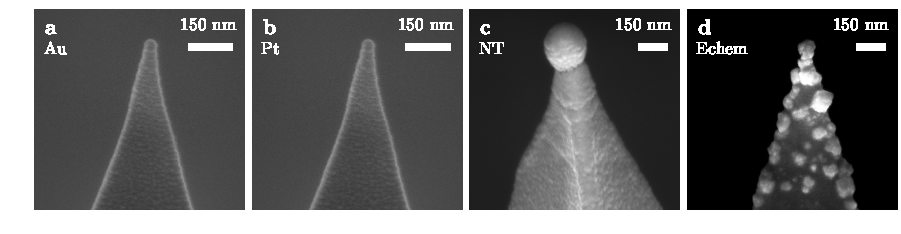
\includegraphics{figures/tip_sems}
\caption[SEM images of sharp and spherical metal tips studied using hyperspectral imaging]{\textbf{SEM images of sharp and spherical metal tips studied using hyperspectral imaging.} Tips are  (a) a sharp Au AFM tip, (b) a sharp Pt AFM tip, (c) a NT Au-coated spherical AFM tip and (d) an electrochemically deposited AuNP-on-Pt AFM tip.}
\label{fig:tip_sems}
\vspace{-10pt}
\end{figure}

% Lead into hyperspectral images and tip comparisons
Hyperspectral images are taken of four different types of AFM probes to investigate the plasmonics of nanostuctured tips. AFM tips studied are Au- and Pt-coated standard AFM probes (BudgetSensors Au-coated AFM probes), spherical Au tips (\SI{300}{nm} Au-coated NanoTools B150 AFM probes) \cite{savage2012} and AuNP-on-Pt AFM probes, fabricated in-house using electrochemical deposition \cite{sanders2014}. SEM images of a selection of these tips are shown in \autoref{fig:tip_sems}. Fabricated tips are pre-treated where possible prior to use with piranha solution to remove organic surface residue and, in some cases, smooth surface roughness. % is the cleaning necessary since this isn't a sub-nm contact paper?

\begin{figure}[bt]
\centering
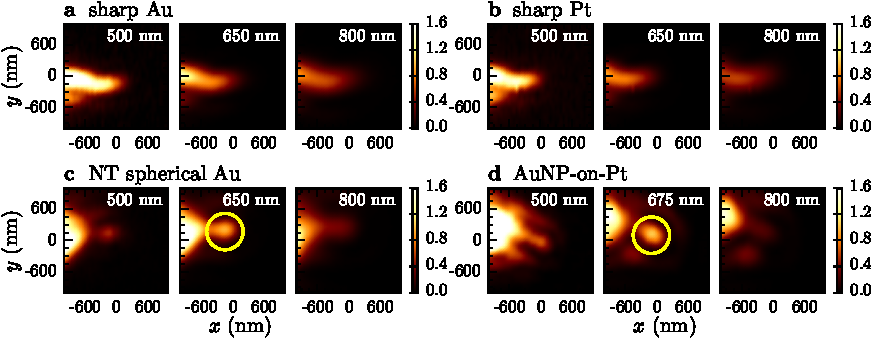
\includegraphics{figures/hyperspectral_tip_comparison}
\caption[Hyperspectral images of sharp and spherical metal tips at wavelengths of interest]{\textbf{Hyperspectral images of sharp and spherical metal tips at wavelengths of interest.} Images are of (a) a sharp Au tip, (b) a sharp Pt tip, (c) a NanoTools Au-coated spherical tip and (d) an electrochemically deposited AuNP-on-Pt tip. Collection polarisation is along the tip axis. Colour maps between slices all have the same normalisation. Resonant scattering from spherical apices is clearly seen in the hyperspectral images of between 600-\SI{700}{nm} and highlighted by yellow circles.}
\label{fig:hyperspectral_tip_comparison}
\vspace{-5pt}
\end{figure}

% Brief description of hyperspectral results
Comparisons between spherical- and sharp-tipped metallic probes using hyperspectral image slices (\figurename~\ref{fig:hyperspectral_tip_comparison}) show that spherical Au tips exhibit a characteristic red (600--\SI{700}{nm}) scatter, delocalised from the bulk tip. No similar localised scattering is seen for sharp Au or Pt tips in the visible spectrum, which have an overall weaker optical response. This delocalised apex scatter can also be clearly seen in wide-field DF imaging.
% Differences between types of spherical tips
The AuNP-on-Pt structure behaves very similarly to the Au-coated diamond-like-carbon spherical tip, likely because the \SI{50}{nm} coating thickness is greater than the skin depth \cite{stockman2011, huber2014}. Plasmons therefore see both as solid Au spheres. Differences in LSPs likely arise due to differences in neck material with Au-Pt and Au-Au neck boundaries.

% Show apex spectra comparison here
\begin{figure}[bt]
\centering
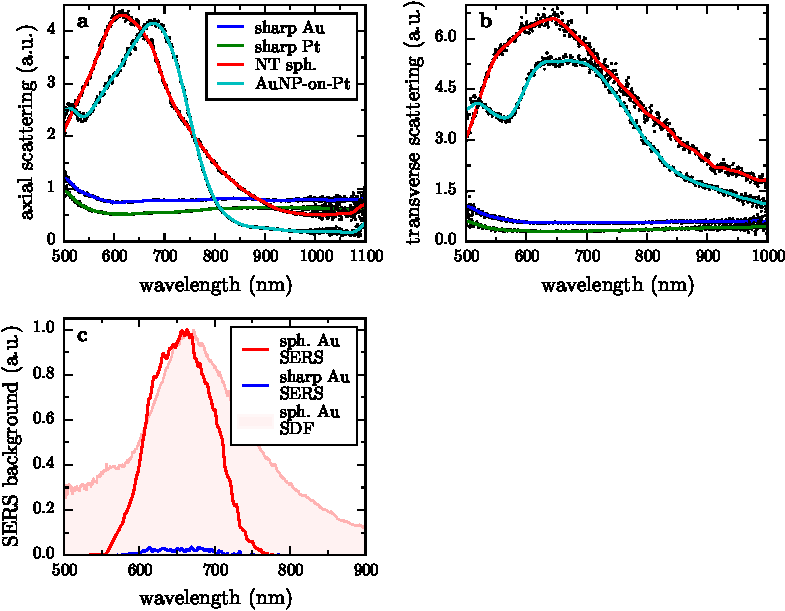
\includegraphics{figures/apex_spectra_comparison}
\caption[Apex spectra of sharp and spherical metal tips]{\textbf{Apex spectra of sharp and spherical metal tips.} Spectra are extracted from the hyperspectral images in \autoref{fig:hyperspectral_tip_comparison} by integrating pixels around the apex region in both the axial (a) and transverse (b) polarisations. A clear resonance between 600--\SI{700}{nm} is observed with spherical tips in both polarisations. Sharp metallic tips show comparatively flat spectra.
Broadband tuneable SERS background measurements of both a sharp and spherical Au tip are integrated across excitation wavelengths spaced \SI{10}{nm} apart (c) to confirm excitation of an LSP. Inelastic scattering of light from the tip apex is plasmonically enhanced in the near-field. The background spectrum is the SDF scattering spectrum of the spherical Au tip apex.
}
\label{fig:apex_spectra}
\vspace{-5pt}
\end{figure}

% Apex spectra comparisons
Integrating spectra around tip apices better shows scattering resonances in spherical Au tips (\figurename~\ref{fig:apex_spectra}a,b), which are reliably present in all spherical-tipped AFM probes, both vacuum-processed and electrochemically deposited. These are attributed to direct LSP excitation. SEM images confirm that this scatter correlates only with spherical Au tip shapes, or when a AuNP is securely attached at the tip apex with a sufficiently small neck joint. The response of sharp Au tips shows no similar plasmonic features while the slow rise in scattering towards the NIR is consistent with lightning rod scattering \cite{zhang2009}.

% Validation of SDF spectra and plasmonic observations
Broadband tuneable SERS \cite{lombardi2015} is used to confirm that the optical resonance seen in spherical Au tips is indeed a LSP by showing that the internal near-field is resonantly enhanced.%
\footnote{Acquisition of broadband tuneable SERS measurements carried out by A.\ Lombardi.}
During plasmon excitation both internal and external fields are enhanced. The external field leads to strong enhancement of Raman spectra whereas inelastic scatter from electrons inside the metal surface is enhanced by the internal plasmonic field, forming the SERS background \cite{hugall2015}. Broadband tuneable SERS is a technique capable of showing both of these components \cite{lombardi2015}. Hence, the near-field plasmon resonance can be calculated by integrating spectra of the SERS background acquired using a range of equally spaced excitation wavelengths.
%\footnote{Model of this behaviour is derived in the appendix.}
SERS background spectra are taken in \SI{10}{nm} increments of the excitation wavelength and integrated between 500--\SI{900}{nm}.
%\footnote{Each acquired background spectrum is shown in the appendix}
The resulting scattering spectrum, shown in \autoref{fig:apex_spectra}c, shows a distinct peak around the spherical Au tip scattering resonance, confirming it as a LSP resonance. Further, confirmation stems from direct observation of plasmon coupling between spherical tips, as has been previously reported \cite{savage2012}, with results of the latest tip coupling experiments discussed in detail in the next chapter.

\FloatBarrier
\subsection{Interpreting the Spectral Response of Metallic Tips}

LSPs in spherical Au tips are \emph{radiative} antenna-like modes, similar to those in spherical AuNPs, that can efficiently couple far-field light into strong collective free electron oscillations without the need for SPP momentum matching. As with AuNPs, the signature of these plasmons is a distinct optical resonance indicating their large dipole moment, as seen in \autoref{fig:apex_spectra}. Such radiative LSPs form only when two close dielectric surfaces surround a metallic particle, allowing for the formation of confined multipolar surface charge oscillations with large dipole moments. Spherical metal tips retain some of the back hemisphere around the connection to the base tip apex (the neck), thus allowing the spherical apex surfaces to sustain similar plasmons. Sharp tips do not have this back surface, hence cannot support such resonances.
Their metal-dielectric surface still, however, supports the launching of evanescent SPPs and a strong lightning rod component.

\begin{figure}[bt]
\centering
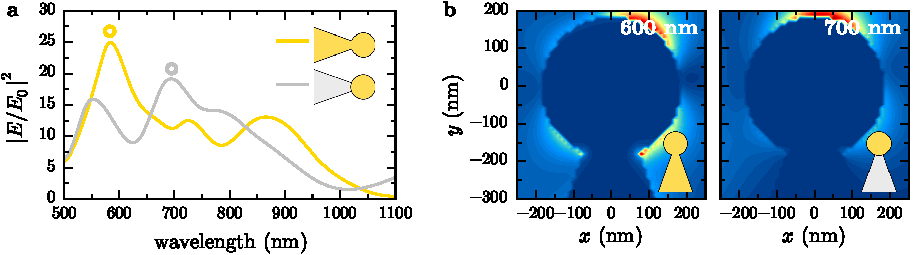
\includegraphics{figures/spherical_tip_simulations}
\caption[Numerical simulations of the field enhancement around a spherical Au tip]{\textbf{Numerical simulations of the field enhancement around a spherical Au tip.} (a) Near-field spectra of spherical Au and AuNP-on-Pt tips, extracted from around the apex of the tip. (b) Near-field enhancement distributions of the two resonances highlighted by circles in (a). Simulated tips have a \SI{300}{nm} spherical radii, \SI{120}{nm} neck widths, \SI{20}{\degree} opening angles and \SI{1.88}{\micro\metre} lengths to best match typical experimental tip geometries. The field is a plane wave orientated along the tip axis.}
\label{fig:spherical_tip_simulations}
\end{figure}

Partial loss of the backside spherical surface and the introduction of a conductive pathway in spherical tips significantly modifies restoring forces and provides a secondary surface for self-interaction. This makes spherical tips difficult to analytically describe. Numerical simulations of the near-field around spherical tips, computed using BEMAX, are instead employed to better understand their response.%
\footnote{BEMAX simulations carried out by D.\,O.\ Sigle.}

Simulated spectra of the near-field around the apices of \SI{300}{nm} spherical Au and AuNP-on-Pt tips with \SI{120}{nm} neck diameters ($d_{\mathrm{neck}}=0.4d_{\mathrm{sphere}}$) are shown in \autoref{fig:spherical_tip_simulations}a. Tips are simulated with a length of \SI{1.88}{\micro\metre} to avoid truncation artefacts and incident fields are orientated along the tip axis. Strong modes appear for both tips between 550--\SI{700}{nm} similar to experiments. The peak positions of the strongest resonance in each tip approximately agree with experimental spectra. Near-field maps corresponding to the main resonance in each tip are shown in \autoref{fig:spherical_tip_simulations}b. The near-field at the dominant resonance in the spherical Au tip appears more quadrupole-like with a weaker dipole-like resonance occurring above \SI{700}{nm}.
Mie theory shows that visible frequency quadrupolar modes are more favourable in larger AuNPs once dipolar resonances shift into the NIR. A similarly structured mode to the AuNP quadrupole plasmon would be expected in \SI{300}{nm} spherical Au tips between 500--\SI{600}{nm}. The neck geometry can also potentially short the pole of dipolar plasmons and reduce their confinement, with quadrupolar charge distributions becoming more favourable.

Similar plasmons are found in the AuNP-on-Pt tip except more blueshifted, with a \SI{700}{nm} resonance appearing more dipole-like and a \SI{550}{nm} resonance appearing more quadrupole-like.
Electromagnetic coupling between Au and Pt surfaces is weaker than the interaction between two Au surfaces \cite{ren2004}, hence plasmons in the spherical Au tip are less redshifted when attached to a Pt tip apex. The non-plasmonic Pt neck region also forms an additional boundary interface to better confine plasmons to the tip. As a result, the dipole-like mode exists nearer to the visible and becomes more favourable than the quadrupole-like mode and easier to couple to. %Failure to experimentally observe the predicted quadrupole-like mode suggests that either the dipolar mode is a far more energetically favourable charge configuration or that the simulated geometry remains too dissimilar to realistic spherical tips. Nevertheless, simulations provide some insight and qualitative descriptions from which to understand plasmons in spherical metallic tips.

\begin{figure}[b]
\centering
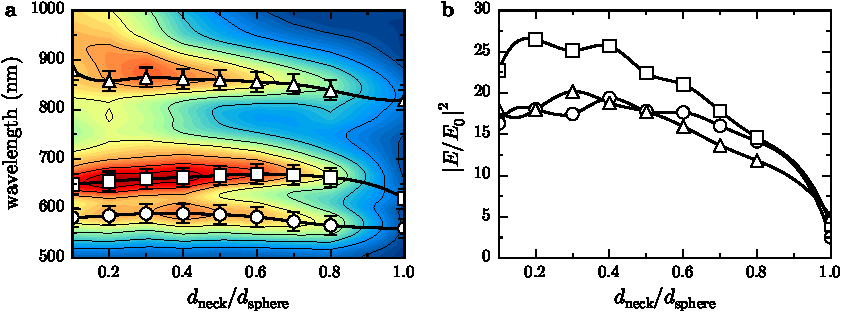
\includegraphics{figures/neck_size_dependence_contour}
\caption[Resonant wavelength and field enhancement dependence on the neck width]{\textbf{Resonant wavelength and field enhancement dependence on the neck width.} The resonant wavelength (a) and field enhancement (b) for each of the resonances present in spherical Au tips as the neck width is varied between that of a spherical tip and a sharp tip. Tips have a \SI{250}{nm} apex diameter, \SI{1.88}{\micro\metre} length, and \SI{10}{\degree} opening angle.}
\label{fig:neck_size_dependence}
\end{figure}

In order to directly compare the \emph{plasmonic} behaviour of spherical Au tips with sharp Au tips, independent of the lightning rod contribution, the neck width is incrementally increased. In this manner, the simulated structure transitions from a AuNP attached to the apex of a sharp Au tip into a rounded tip geometry, similar in shape to a sharp Au tip, without the apex radius ever changing.
%{\color{red}A smaller radius of curvature and opening angle are used to fall between the expected behaviour of both sharp and spherical tips.}
The field enhancement and peak positions extracted from this morphology transition are shown in \autoref{fig:neck_size_dependence}. Resonances are insensitive to the neck width until it becomes greater than $0.8d_{\mathrm{sphere}}$, explaining the robustness of observed spherical tip plasmons between different tip morphologies. A steady decrease in the field enhancement, however, is observed once $d_{\mathrm{neck}}>0.4d_{\mathrm{sphere}}$, decreasing faster once $d_{\mathrm{neck}}>0.8d_{\mathrm{sphere}}$. This supports the claim that sharp tips cannot sustain antenna-like LSPs.

\subsection{Implications of Spherical Metallic Tip Plasmonics}

The presented results demonstrate the importance of considering what plasmons might exist in a particular experiment and nanostructure geometry, and that it is vital to characterise nanostructures prior to their application in any further techniques. Without prior knowledge as to where in the visible spectrum plasmons are excited it is difficult to properly interpret any measurements, such as TERS spectra. Improved tip characterisation is crucial to understanding why such varied TERS enhancements are reported. Standard, wide-field microscopy is not a particularly effective tool for optically characterising tips. Confocal hyperspectral imaging, instead, provides a viable method for mapping the local scattering response with broadband tuneable SERS offering a unique way of optically characterising the near-field.

Exploiting visible LSPs in spherical tips also permits the use of a wider range of illumination configurations as the restriction to evanescent coupling is lifted. Regardless of plasmonics, the lightning rod effect will always play a role in the near-field enhancement process, giving sharp tips an initial advantage, but with careful optimisation of the spherical tip geometry, tips can be brought into resonance with a laser wavelength to maximise enhancement. Spherical Au tips in their current form are already quite well optimised for TERS due to being on resonance with the readily available \SI{633}{nm} HeNe laser wavelength often used.

Plasmons in spherical tips have also been shown to readily couple with plasmons in other spherical tips \cite{savage2012} and would be expected to couple with image charges in a planar mirror, thus significantly increasing their near-field enhancement. In this situation, their resonances can be tracked as the tip approaches the surface and stopped on resonance with the incident TERS laser for maximum enhancement, for example at the common \SI{785}{nm} excitation wavelength. For small gaps on the nanometre level, the plasmon mode will become strongly confined to the gap and its contribution to the near-field could outweigh the lightning rod effect.
Exploiting radiative tip plasmons in this manner bridges the gap between the plasmonics involved in SERS and TERS. Some of the largest enhancement factors recently measured in plasmonic systems originate from radiative plasmons in AuNPs coupled with their image charge distribution in a mirror \cite{mertens2013, taylor2014}. These systems repeatedly produce Raman enhancements of up to $10^7$ with nanometric mode volumes, much like tips, demonstrating that plasmonic gaps can exhibit large field enhancement without requiring a significant contribution from the lightning rod effect. However, the static nature of the NPoM geometry lacks the ability to chemically map a surface. By coupling plasmons in spherical tips with their mirror charge, surfaces could be dynamically mapped with a potentially very large field enhancement.

This discussion on single tip plasmonics is concluded by performing one measurement specifically relevant to TENOM. To demonstrate the advantages of having prior knowledge of excited plasmons in tips, along with the advantages of using AuNP-on-Pt tips, a TERS measurement is performed directly after characterisation on resonance with a plasmon.

\end{document}